\chapter{Two Languages: Lean 4 and rusty-SUNDIALS}\label{ch02}

\section{Two ways to be wrong}\label{ch02:wrong}

The first run of the registered controls of the programme's solver for the projected Gross--Pitaevskii equation (PGPE), recorded in an amendment dated 22 September 2026, reported that the
total momentum of an isolated, periodic, two-dimensional fluid had changed by $8.54$ in $20$ time units, one per cent of its value, and had done so identically at two
different time steps. Momentum cannot change in such a system, since translating the periodic box leaves the equation unchanged; and a drift that does not depend on the step is not a
fault of the time stepping but of the equation being stepped. The same run, which tests the norm (control K1), the energy (K2), the momentum (K3) and an exact plane-wave solution (K4),
had found the norm conserved to $4.2\times10^{-10}$ and the plane wave reproduced to $7.0\times10^{-10}$: those two controls passed, and neither could have seen the fault. It sat in a sentence of the
programme's own pre-registration, which said that a cutoff at two thirds of the largest wave number makes the cubic term of the equation free of aliasing. That is the rule for a quadratic
nonlinearity \cite{Orszag1971}; for a cubic term the cutoff has to sit at one half. The aliased scheme is not translation invariant, and the momentum control saw it.\footnote{Amendment~A1 of the programme's pre-registration
(\texttt{docs/designs/PGPE\_BKT\_PREREG.md}, 2026-09-22) and the stored first run \texttt{data/generated/pgpe/known\_answers.json}: $N=64$, $L=32$, a random state of energy $3$ per particle,
$t=20$, momentum drift $8.5358$ at $\Delta t=0.005$ and $8.5358$ at $0.01$. The numbers of this paragraph are quoted from those files, not recomputed.}

A different kind of fault is the subject of a remark in the 2021 paper by Godfrin and his co-authors on the dispersion relation of superfluid
helium-4 \cite{Godfrin2021}. Equation~(22) of that paper gives the phonon specific heat as a series,
$C_V=AT^3+CT^5+DT^6+ET^7+KT^8+LT^9$, and the authors note that earlier published versions of the series contain errors.
The neutron measurement fixes the dispersion relation; the step from the dispersion to the series is algebra, and a formula of that length is
exactly where a coefficient or a sign can be wrong without anyone noticing.

\begin{godfrinbox}{A printed series, and a remark about it}
The inelastic neutron-scattering measurement of Godfrin, Beauvois, Sultan, Krotscheck, Dawidowski, F\aa k and Ollivier on superfluid $^4$He
(spectrometer IN5, Institut Laue--Langevin; Phys.\ Rev.\ B \textbf{103}, 104516 (2021)) gives the Landau phonon--maxon--roton dispersion (the authors' published table runs
from $0$ to $3.6\,\text{\AA}^{-1}$) and the thermodynamic consequences. Its Eq.~(22) is the series above, for a dispersion
$\varepsilon=\hbar ck\,(1+\alpha_2k^2+\dots+\alpha_6k^6)$ with $\alpha_1=0$, and the paper remarks that earlier versions of this series contain errors.
The programme re-derived the series independently and proved all six coefficients in Lean. That is a \emph{confirmation of the printed formula},
not a finding, and a proof of a mathematical statement, not of the experiment; \cref{ch04} tells it.
\end{godfrinbox}

The two faults call for two different instruments, and this chapter is a primer on both. The second fault, an algebraic slip, is the business of a
proof assistant: a computer checks the derivation, and a wrong coefficient cannot pass. The first fault is not. The programme had a Lean theorem about the
cubic term, and the theorem was true; it was about the \emph{exact} Galerkin convolution on an additive group such as the integer lattice, while the program evaluated a
different function, a fast Fourier transform on a periodic grid, which coincides with the convolution only when no triple of wave vectors wraps around the
grid. A proof checks a statement against its hypotheses and a simulation checks a program against an expectation; neither checks that the program computes
the object the statement is about.

\begin{keybox}[The division of labour]
A theorem is about a \emph{function}; a run is of a \emph{program}. Lean can establish that the function has a property for every state and every
parameter. The solver can show that the program reproduces an exact solution, an independent integrator or a conservation law to a stated precision, in a stated
case. Each instrument is blind where the other sees, and the instructive cases are those in which they disagree.
\end{keybox}

We follow one equation through both languages. \Cref{ch02:lean} is Lean in twenty minutes; \cref{ch02:theorem} states the theorems that concern the
equation; \cref{ch02:solver} is the solver in twenty minutes; \cref{ch02:known,ch02:planewave,ch02:alias} are three experiments, the last of
which is the fault above, reproduced and measured; \cref{ch02:see} sorts out which instrument can see what.

\section{Lean 4 in twenty minutes}\label{ch02:lean}

Lean~4 \cite{deMoura2021} is at once a programming language and a proof assistant. In it a statement is a \emph{type}, a proof of the statement is a
\emph{term} of that type, and a small program, the \emph{kernel}, checks that the term has the type it is claimed to have. The kernel, together with the axioms
it is told to assume, is what a reader has to trust; the elaborator and the tactics that build terms are not trusted, because whatever they produce is
re-checked. Mathlib \cite{Mathlib2020} is the community library of mathematics on which the programme builds. The programme's own library, \lean{QuantumFluids},
adds 37 modules with 310 theorems and lemmas (413 declarations in all) on the mathematics of quantum fluids, compiled with Lean 4.34.0-rc2 against the matching
Mathlib; its sources are in \texttt{lean\_src/}. Every statement quoted from it in this book is copied from there and cited by module and name.
The Lean written for this chapter is marked \emph{new} in the title of its box, lives in \texttt{book/lean/}, and was compiled with zero errors and no \lean{sorry};
the \lean{\#print axioms} lines quoted below are those of the compiler.

The box below contains the whole vocabulary needed to read a Lean statement.

\begin{leanbox}{new: Ch02\_Primer}
\begin{lstlisting}[style=lean]
#check (2 : ℕ)                  -- 2 : ℕ
#check (2 + 2 = 4)              -- 2 + 2 = 4 : Prop
example : 2 + 2 = 4 := rfl      -- a proof is a term of that type

theorem and_swap' (p q : Prop) (hp : p) (hq : q) : q ∧ p :=
  ⟨hq, hp⟩

theorem two_add_two : (2 : ℝ) + 2 = 4 := by norm_num

theorem one_add_nilpotent_inv {R : Type*} [CommRing R]
    (e : R) (h : e ^ 2 = 0) : (1 + e) * (1 - e) = 1 := by
  linear_combination (-1 : R) * h
\end{lstlisting}
\end{leanbox}

The first two lines ask Lean for the type of an expression: \lean{2} is a natural number, and \lean{2 + 2 = 4} is a proposition, an element of the type \lean{Prop}.
The line \lean{example : 2 + 2 = 4 := rfl} proves it: both sides reduce to the same numeral, so reflexivity of equality is a proof. The theorem \lean{and\_swap'} says
that if two propositions hold then they hold in the other order; its proof is the pair \lean{⟨hq, hp⟩}, a term written by hand. The theorem
\lean{two\_add\_two} is about real numbers, and its proof is a \emph{tactic}: \lean{norm\_num} searches for a proof and hands the result to the kernel.

The last theorem is the pattern the library uses at scale. In any commutative ring \lean{R} with an element \lean{e} satisfying \lean{e \^{} 2 = 0}, the element
\lean{1 + e} has the inverse \lean{1 - e}. The tactic \lean{linear\_combination (-1 : R) * h} is a \emph{certificate}: it asserts that the goal, minus $-1$ times the
hypothesis \lean{h}, is an identity of commutative rings, and \lean{ring} checks that identity. The certificate was supplied from outside and the kernel checks it;
nothing about how it was found has to be believed. The module \lean{PhononSeries} uses exactly this pattern for the series of the previous
section: its certificates, computed by computer algebra, run to several thousand characters per line (see \Lthm{PhononSeries}{kPow2_eq}) and are checked by the
kernel like the toy above. Truncating a power series at order $e^8$ becomes the statement \lean{e \^{} 8 = 0} in a commutative ring, with no analysis needed.

\paragraph{What the kernel refuses.} A checker is only worth having if it can say no. With the coefficient of the certificate mistyped (\lean{(1 : R)} instead of \lean{(-1 : R)}),
the same tactic refuses; and so does \lean{norm\_num} on a false numerical statement. The compiler's reply to the file \texttt{book/lean/Ch02\_NegativeControl.lean}, which exists only to be refused
(file path shortened, and the hygiene mark that Lean prints after \lean{inst} omitted):
\begin{lstlisting}[style=plainmono]
Ch02_NegativeControl.lean:9:2: error: ring failed, ring expressions not equal
R : Type u_1
inst : CommRing R
e : R
h : e ^ 2 = 0
⊢ -(e ^ 2 * 2) = 0
Ch02_NegativeControl.lean:12:29: error: unsolved goals
⊢ False
\end{lstlisting}
The residual $-2e^2$ is the evidence: with the wrong sign the goal minus the certificate is not zero as a ring identity (the goal needed $-e^2$ and the certificate supplied $+e^2$), and no proof
is produced. The second error is \lean{norm\_num} reducing \lean{2 + 2 = 5} to \lean{False}.

\paragraph{What an axiom audit looks like.} A Lean file can end with a line \lean{\#print axioms} for each theorem, which lists the axioms the proof ultimately depends on; the library files carry such lines (written by a script), and Appendix~\ref{appA} tabulates the
audit of every module. The file of the box above prints
\begin{lstlisting}[style=plainmono]
'QuantumFluids.Ch02Primer.and_swap'' does not depend on any axioms
'QuantumFluids.Ch02Primer.two_add_two' depends on axioms: [propext, Classical.choice, Quot.sound]
'QuantumFluids.Ch02Primer.one_add_nilpotent_inv' depends on axioms: [propext, Quot.sound]
\end{lstlisting}
The three names are the standard foundation of classical mathematics in Lean and Mathlib (propositional extensionality, the axiom of choice, soundness of quotients);
\lean{and\_swap'} needs no axiom at all, and the certificate needs two. An incomplete proof shows up as a fourth name, \lean{sorryAx}: when the first draft of this chapter's Lean file
contained a proof that did not compile, the compiler reported the error and replaced the proof by \lean{sorry}, and the audit lines of the two theorems that depended on it read
\lean{[propext, sorryAx, Classical.choice, Quot.sound]}. That line is the reason the audit exists.

\paragraph{A program is not a theorem.} Lean also runs programs. The three commands
\begin{lstlisting}[style=lean]
#eval (List.range 6).map (fun n => n ^ 2)
#eval (0.1 + 0.2 : Float)
#eval ((0.1 + 0.2 : Float) == 0.3)
\end{lstlisting}
print, in that order,
\begin{lstlisting}[style=plainmono]
[0, 1, 4, 9, 16, 25]
0.300000
false
\end{lstlisting}
\lean{Float} is the machine's double-precision number, the same 64-bit format as \texttt{float64} in numpy and \texttt{f64} in Rust, and in it the sum of $0.1$ and $0.2$ is
not $0.3$. In the same file the theorem \lean{(1 / 10 + 2 / 10 : ℝ) = 3 / 10} is proved by \lean{norm\_num}, because in the field of real numbers the equation is exact.
A theorem about \lean{ℝ} is a statement about mathematics; what a program returns is a statement about a finite machine. Nothing in the library speaks about the rounding of
any program, and that is why the solver of this book is checked by experiment and the equation by proof.

\section{A theorem about the equation the solver integrates}\label{ch02:theorem}

The projected Gross--Pitaevskii equation \cite{Davis2001,Blakie2008} is the classical-field description of a Bose fluid used throughout the programme. In units $\hbar=m=1$, on a
periodic box of side $L$,
\begin{equation}\label{ch02:eq-pgpe}
 \ii\,\partial_t\psi \;=\; P\Bigl[-\tfrac12\nabla^2\psi+g\,|\psi|^2\psi\Bigr],
\end{equation}
where $P$ keeps the Fourier modes with $|k|\le k_{\rm cut}$ and discards the others. Writing $\psi(x,t)=\sum_{k\in\Lambda}a_k(t)\,\ee^{\ii k\cdot x}$ with $k=2\pi n/L$, $n\in\mathbb Z^2$, and
$\Lambda$ the finite set of retained modes, the equation becomes a system of ordinary differential equations,
\begin{equation}\label{ch02:eq-modes}
 \ii\,\dot a_k=\omega_k\,a_k+g\,N_k(a),\qquad \omega_k=\tfrac12|k|^2,\qquad
 N_k(a)=\sum_{\substack{k_1,k_2,k_3\in\Lambda\\ k_1+k_3=k+k_2}}a_{k_1}\,\overline{a_{k_2}}\,a_{k_3},
\end{equation}
for $k\in\Lambda$. This is the system that the Lean module \lean{GPGalerkin} is about, with an arbitrary additive group in place of $\mathbb Z^2$ and an arbitrary finite
set $\Lambda$ (nothing in what follows depends on which modes are retained), and with the amplitudes called $\psi_k$ and the integer vectors $n$ as the elements of the group (the factor $2\pi/L$ sits in $\omega$). The box below quotes its definition of $N$ and two of its theorems.

\begin{leanbox}{GPGalerkin}
\begin{lstlisting}[style=lean]
-- variable {G : Type*} [AddCommGroup G] [DecidableEq G]

noncomputable def nl (Λ : Finset G) (ψ : G → ℂ) (k : G) : ℂ :=
  ∑ k1 ∈ Λ, ∑ k2 ∈ Λ, ∑ k3 ∈ Λ,
    if k1 + k3 = k + k2 then ψ k1 * (starRingEnd ℂ) (ψ k2) * ψ k3 else 0

theorem pairing_eq_sum (Λ : Finset G) (ψ : G → ℂ) :
    pairing Λ ψ =
      ∑ q ∈ diffs Λ, dens Λ ψ q * (starRingEnd ℂ) (dens Λ ψ q) := by
  -- (proof abridged) rearrangement of finite sums

theorem mass_rate_zero (Λ : Finset G) (ψ : G → ℂ) (ω : G → ℝ)
    (g : ℝ) :
    ∑ k ∈ Λ,
      ((starRingEnd ℂ) (ψ k) *
        ((ω k : ℂ) * ψ k + (g : ℂ) * nl Λ ψ k)).im = 0 := by
  -- (proof abridged) termwise, conj ψ_k * (ω_k ψ_k + g N_k) is
  -- the real number ω_k |ψ_k|² plus g * (conj ψ_k * N_k); the
  -- second parts sum to g * pairing Λ ψ, whose imaginary part is
  -- 0 (pairing_im_zero): pairing Λ ψ is a sum of squared moduli
\end{lstlisting}
\end{leanbox}

The symbols: \lean{Finset G} is a finite subset of the group \lean{G}; \lean{∑ k ∈ Λ, f k} is the finite sum; \lean{starRingEnd ℂ} is complex conjugation; \lean{.im} is the imaginary part;
\lean{(ω k : ℂ)} is a real number regarded as a complex one. The definition \lean{nl} is the sum of \cref{ch02:eq-modes}, with the condition
$k_1+k_3=k+k_2$ written as an \lean{if}. The theorem \Lthm{GPGalerkin}{pairing_eq_sum} says that the quartic interaction sum $Q=\sum_k\overline{\psi_k}N_k$ equals $\sum_q|A_q|^2$, where
$A_q=\sum_{a-b=q}\psi_a\overline{\psi_b}$ is the Fourier transform of the density $|\psi|^2$; hence $Q$ is real and non-negative (\Lthm{GPGalerkin}{pairing_nonneg}), which
is the defocusing sign of the interaction, for every $\Lambda$. The theorem \Lthm{GPGalerkin}{mass_rate_zero} is the algebraic core of the conservation of the norm: for
$\ii\dot\psi_k=G_k$ one has $\mathrm d|\psi_k|^2/\mathrm dt=2\,\mathrm{Im}(\overline{\psi_k}G_k)$, so the theorem says that the \emph{rate} of change of $\sum_k|\psi_k|^2$ is zero.
The whole conservation law is the statement that a certain sum is real, and the abridged proof says why. (All thirteen theorems of the module depend on the three standard axioms and on nothing else, as the audit lines at the end of the file show.)

What the theorem does not say is as important. It does not say that the system has a solution, or that the solution is unique; it does not say that
$\sum_k|\psi_k|^2$ is constant along a solution (that needs the chain rule, which the library does not formalize); and it says nothing about the numbers that any
integrator returns. The companion statement for the energy, \Lthm{GPGalerkin}{energy_rate_zero}, is of the same kind: an algebraic core, with the same limits, resting on the gradient identity
\Lthm{GPGalerkin}{grad_identity}.

The library has no statement about the third conservation law of this equation, momentum. The programme's pre-registration of the solver (its section~4) said otherwise: it
stated that the invariants of the controls K1 to K3 were theorems of \lean{GPGalerkin} and that the projector did not change them. Two of the three were
there as algebraic cores only, and the third was not there at all. The fault of \cref{ch02:wrong} was in the second half of that sentence. The statements written for this chapter
repair the first half; \cref{ch02:alias} measures the second.

\begin{leanbox}{new: Ch02\_Galerkin}
\begin{lstlisting}[style=lean]
-- variable {G : Type*} [AddCommGroup G] [DecidableEq G]
-- nl : as in GPGalerkin, copied verbatim

noncomputable def planeWave (a₀ : ℂ) (ω t : ℝ) : ℂ :=
  a₀ * Complex.exp (-(Complex.I * ω) * t)

noncomputable def planeState (k0 : G) (a₀ : ℂ) (Ω t : ℝ) :
    G → ℂ :=
  fun x => if x = k0 then planeWave a₀ Ω t else 0

noncomputable def galerkinField (Λ : Finset G) (ω : G → ℝ)
    (g : ℝ) (ψ : G → ℂ) (k : G) : ℂ :=
  -Complex.I * ((ω k : ℂ) * ψ k + (g : ℂ) * nl Λ ψ k)

theorem planeState_solves_galerkin (Λ : Finset G) (k0 : G)
    (hk0 : k0 ∈ Λ) (ω : G → ℝ) (g : ℝ) (a₀ : ℂ) (k : G)
    (t : ℝ) :
    HasDerivAt
      (fun s : ℝ =>
        planeState k0 a₀ (ω k0 + g * ‖a₀‖ ^ 2) s k)
      (galerkinField Λ ω g
        (planeState k0 a₀ (ω k0 + g * ‖a₀‖ ^ 2) t) k) t := by
  -- (proof abridged) nl of a one-mode state is |a|² a on that
  -- mode and 0 elsewhere (nl_single); on the mode, |planeWave|
  -- is constant and planeWave' = -i Ω planeWave
\end{lstlisting}
\end{leanbox}

\paragraph{The exact plane wave.} The box above states the solution on which the programme's fourth known answer (K4) rests.
A single occupied mode $k_0$ with amplitude $a_0\,\ee^{-\ii\Omega t}$, where $\Omega=\omega_{k_0}+g|a_0|^2$, solves the Galerkin system on every finite mode set that contains $k_0$, for
every dispersion $\omega$, every coupling $g$ and every amplitude. The theorem evaluates the vector field of \cref{ch02:eq-modes} on the plane-wave state, component by component, and equates it
to the time derivative of that component. It is a statement about $\mathbb R$ and $\mathbb C$ and about no program; \cref{ch02:planewave} asks three integrators to reproduce it.

\begin{leanbox}{new: Ch02\_Galerkin}
\begin{lstlisting}[style=lean]
theorem momentum_rate_zero (Λ : Finset G) (ψ : G → ℂ)
    (ω : G → ℝ) (g : ℝ) (p : G →+ ℝ) :
    ∑ k ∈ Λ, p k * ((starRingEnd ℂ) (ψ k) *
      ((ω k : ℂ) * ψ k + (g : ℂ) * nl Λ ψ k)).im = 0 := by
  -- (proof abridged) the four-fold sum over (a, b, c, d) with
  -- b + d = a + c of p a * conj ψ_a ψ_b conj ψ_c ψ_d; the
  -- renamings a<->c, b<->d, (a,b,c,d)->(b,a,d,c); additivity:
  -- p a + p c = p (a + c) = p (b + d) = p b + p d; so it is real

theorem no_momentum_on_torus (N : ℕ) [NeZero N]
    (p : (ZMod N × ZMod N) →+ ℝ) (x : ZMod N × ZMod N) :
    p x = 0 := by
  -- (proof abridged) N • x = 0 in the torus, so N * p x = 0 in ℝ
\end{lstlisting}
\end{leanbox}

\paragraph{Momentum, and the hypothesis that carries it.} The box above is the new statement behind the fault of \cref{ch02:wrong}. Here \lean{p : G →+ ℝ} is an \emph{additive map}: $p(k+k')=p(k)+p(k')$.
On $G=\mathbb Z^2$ these are exactly the linear combinations of the two components of the wave vector, so \lean{momentum\_rate\_zero} says that the rate of change of the total momentum
$\sum_k p(k)\,|\psi_k|^2$ vanishes, for every finite $\Lambda$ and every state. The constant weight $p\equiv1$ is not additive (the norm has its own theorem and proof); the momentum theorem uses, besides the resonance condition $k_1+k_3=k+k_2$, \emph{only} that $p$ is additive. The abridged proof is short. The nonlinear part of the momentum rate is
the imaginary part of the four-fold sum $S_a=\sum p(a)\,\overline{\psi_a}\psi_b\overline{\psi_c}\psi_d$ over quadruples with $b+d=a+c$. Renaming $a\leftrightarrow c$ leaves the summand unchanged, so
$S_a=S_c$, and likewise $S_b=S_d$ when the weight is $p(b)$ or $p(d)$; additivity and the resonance condition give $p(a)+p(c)=p(b)+p(d)$, so $S_a+S_c=S_b+S_d$ and therefore $S_a=S_b$; and
complex conjugation maps the summand at $(a,b,c,d)$ to the summand at $(b,a,d,c)$, so $\overline{S_a}=S_b=S_a$. A number equal to its conjugate is real. In the file the three renamings are
three short chains of \lean{Finset.sum\_comm}, and the last step is one \lean{linear\_combination}; a corollary instantiates $G=\mathbb Z\times\mathbb Z$ and $p(k)=k_1$.

The second theorem of the box says why the hypothesis is not decoration. On the periodic grid $\mathbb Z_N\times\mathbb Z_N$, where the engine's wave vectors live, every additive map to the real numbers is
zero: there is no additive momentum, so \lean{momentum\_rate\_zero} has no content there. This does \emph{not} prove that momentum fails to be conserved by a wrapped-around scheme (that is a
measurement, \cref{ch02:alias}); it says that the proof has nothing to stand on. It follows (\lean{no\_additive\_wavenumber} in the file) that the wave number itself, $k\mapsto k$, is not an additive
function modulo $N$, which is the formal form of ``aliasing breaks translation invariance''.

\section{rusty-SUNDIALS in twenty minutes}\label{ch02:solver}

\paragraph{What CVODE does.} CVODE integrates $y'=f(t,y)$, $y(t_0)=y_0$, by linear multistep methods: the new value is built from several previous values and from $f$, with a step $h$ and
an order $q$ that the solver changes as it goes. Two families are offered. The Adams--Moulton methods (orders 1--12) are meant for smooth, non-stiff problems and the backward differentiation formulas
(BDF, orders 1--5) for stiff ones. Both are implicit, the new value appears on both sides, and in the Rust implementation both are solved by the same Newton iteration with a dense LU factorization of
$I-\gamma J$; when the user supplies no Jacobian, as in the Python module, $J$ is built column by column by finite differences, at the price of $n$ extra evaluations of $f$ per Jacobian for a system of
dimension $n$. The solution is kept as a Nordsieck array of scaled derivatives. After each step the solver estimates the local error from the size of the Newton correction,
weights it component by component with $1/(\mathrm{rtol}\,|y_i|+\mathrm{atol})$, accepts or rejects the step, and chooses $h$ and $q$ for the next one. The user states a tolerance, not a step. What the
tolerance controls is the \emph{local} error of each step; the error of the final answer is not guaranteed to be of that size, and \cref{ch02:known} shows how far it can stray.

\paragraph{What rusty-SUNDIALS is.} rusty-SUNDIALS is the programme's Rust implementation of this algorithm, translated, in the words of its source files, from the C code of the SUNDIALS suite \cite{Hindmarsh2005}. The Python
module \texttt{rusty\_sundials} exposes one class, \lean{CvodeSolver(method, rtol, atol, max\_steps)}, with one method, \lean{solve(rhs, t0, y0, t\_out)}, which calls the user's Python function \lean{rhs(t, y)} and
returns the pair $(t,y)$ at the end of the interval and nothing else; a trajectory is obtained by many calls, and every call starts the integration afresh. The Rust source calls the order selection of its BDF path a simple heuristic, so step counts need not match those of the C code, and its repository's README speaks of Lean~4 specifications of the solver that this book
neither uses nor re-checks. Nothing in this book is a proof about the Rust code. It is tested: against closed-form solutions, against a second integrator of the same equation, and against the programme's
numpy implementation of the engine. The word ``verified'' in the title of the software paper \cite{Callens2026sw} is used in that sense: its claims are agreements with reference answers, listed there with their precision.

\begin{rustbox}{CVODE from Python}
% CODE snippet1
\begin{lstlisting}[style=py]
import math
from rusty_sundials import CvodeSolver

calls = 0
def rhs(t, y):
    # x'' = -x written as a first-order system (x, v)
    global calls
    calls += 1
    return [y[1], -y[0]]

T = 20 * math.pi        # ten periods; the exact solution is (cos T, -sin T)
for method in ("adams", "bdf"):
    calls = 0
    # arguments: method, rtol, atol, max_steps
    solver = CvodeSolver(method, 1e-8, 1e-10, 100000)
    t, y = solver.solve(rhs, 0.0, [1.0, 0.0], T)
    err = max(abs(y[0] - math.cos(T)), abs(y[1] + math.sin(T)))
    print(f"{method:5s} rhs calls {calls:6d}  error {err:.2e}")
\end{lstlisting}
% OUTPUT snippet1
\begin{lstlisting}[style=plainmono]
adams rhs calls   1549  error 3.76e-07
bdf   rhs calls   5217  error 2.53e-06
\end{lstlisting}
Output of \texttt{figures/ch02\_snippets.py}, run with the module described below.
\end{rustbox}

The box above is the whole interface in use: ten periods of the harmonic oscillator, both methods, the exact answer known. The number of calls of \lean{rhs}, which includes the columns
of the finite-difference Jacobian, is the \emph{cost} used throughout this chapter; unlike wall time it does not depend on the load of a shared machine. Both runs asked for a relative tolerance of $10^{-8}$,
and neither delivered a final error of that size: $3.8\times10^{-7}$ and $2.5\times10^{-6}$.

\paragraph{A defect, and a stale build.} Until it was repaired, \lean{Method::Adams} never left order~1: the coefficients that define the higher orders were placeholders, so every Adams run was implicit Euler
with an error estimate of the wrong kind, and under a per-step error control a first-order method has a global error that falls only as the square root of the tolerance. The defect was first seen as exactly that
square-root convergence on a cosmological distance integral, and it also blocks the programme's order test of the PGPE engine against CVODE (\cref{ch02:planewave}), which cannot finish without the repair: the Adams path
fails after about $10^6$ evaluations. The repair implements the order and step selection of the C library (rusty-SUNDIALS, \texttt{docs/CVODE\_ADAMS\_FIX.md}, dated 2026-09-28). The Python module in the
programme's virtual environment was built on 26 September, before it, and still has the defect. This chapter's first probe, run with that module, showed the old signature at once; every CVODE result below comes from a build of the checked-out
sources (commit \texttt{5db8041}, release line v11.6.0), and the compute script refuses to run with a module whose Adams path takes more than $5\,000$ evaluations on $y'=-y$.
Panel~(d) of \cref{ch02:fig-workprec} shows the two builds side by side.

\paragraph{What qf-pgpe is.} The quantum-fluids crate \texttt{qf-pgpe} integrates \cref{ch02:eq-pgpe} on a periodic grid by an integrating-factor Runge--Kutta scheme of order four (IF-RK4): the linear part
$-\ii k^2/2$ is applied exactly in Fourier space, the cubic part by classical RK4, the projector is a sharp circle at $k_{\rm cut}=k_{\max}/2$, and the arrays follow numpy's FFT conventions so that the
Python programme and the Rust engine exchange fields without conversion. A Python extension, \texttt{qf\_pgpe}, runs a whole time interval in one call. The same right-hand side is available to external integrators as a
system of $2n_{\rm modes}$ real equations (the functions \lean{rhs}, \lean{pack} and \lean{unpack} of the engine): that is how CVODE enters, as a second integrator, written independently, of the \emph{identical}
equation. On the programme's benchmark the single-threaded Rust step is $4.3$, $4.2$, $2.7$ and $2.5$ times faster than the numpy step at $N=64$, $128$, $256$ and $512$ \cite{Callens2026sw}; those
numbers were measured on a 2013 four-core laptop processor shared with an unrelated job, and are quoted, not repeated here. The dense Jacobian of the Python module needs $n$ evaluations and $n^2$ numbers of memory for
$n=2n_{\rm modes}$: for the $128^2$ grid of the thermal sweep ($\approx3\,200$ modes) about $330$\,MB. CVODE is therefore used here as a referee on a $16\times16$ grid ($49$ modes,
$n=98$), not as the production integrator. No GPU code is involved anywhere in this book.

\section{The solver on problems with known answers}\label{ch02:known}

Before asking CVODE anything about a quantum fluid we ask it questions to which we know the answers. \Cref{ch02:fig-stab} is the theory behind the questions. For the test equation $y'=\lambda y$ a
multistep formula with the step frozen advances $y$ by an amplification factor determined by $z=h\lambda$; the \emph{region of absolute stability} is the set of $z$ for which the factors do not grow
\cite{Dahlquist1963,HairerWanner1996}. For the Adams--Moulton formulas of order three and higher the region is a small lobe around the origin, with intercepts on the negative real axis of $-6.00$, $-3.00$, $-1.84$
and $-1.18$ for orders 3 to 6 (computed here, not copied); the trapezoidal rule and implicit Euler are stable on the whole left half-plane. For BDF the unstable region is a bounded lobe on the right, and every
point outside it is stable. BDF of orders 1 and 2 are stable on the whole left half-plane; orders 3, 4 and 5 are stable in a wedge of half-angle $\alpha=86.0^\circ$, $73.4^\circ$ and $51.8^\circ$ around the negative real axis and
leave out a wedge of the left half-plane next to the imaginary axis, which widens with the order. A problem is \emph{stiff} when its eigenvalues have large negative real parts: then any step that resolves the solution has $h\lambda$ far outside an
Adams lobe, and only a formula whose region contains the far left half-plane (BDF, or the Adams formulas of orders 1 and 2) can take it with a step that accuracy, not stability, chooses.

\begin{figure}[tp]\centering
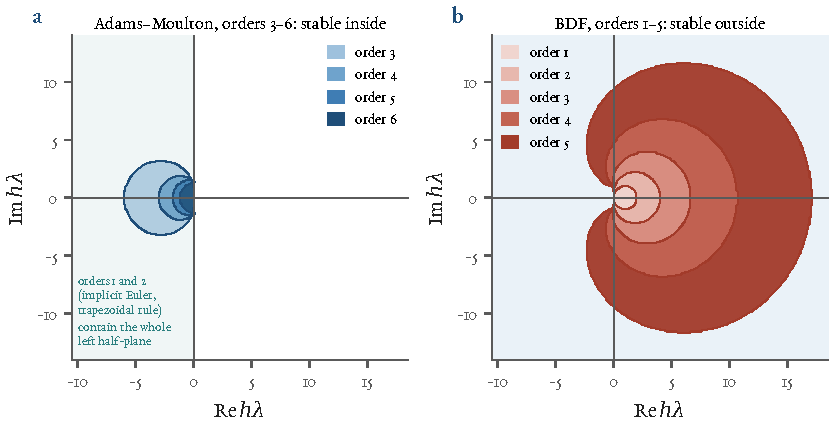
\includegraphics[width=\linewidth]{figures/ch02_stability.pdf}
\caption[Regions of absolute stability of the Adams and BDF formulas]{Regions of absolute stability, computed by a root test on a grid of $z=h\lambda$ for the fixed-step formulas to which CVODE's two families reduce when step and order are frozen.
(a) Adams--Moulton, orders 3--6: stable inside the lobes; orders 1 and 2 (implicit Euler, trapezoidal rule) are stable on the whole shaded left half-plane.
(b) BDF, orders 1--5: the filled lobes are the \emph{unstable} regions, everything else is stable. The coefficients were checked against their order conditions (exactness on polynomials), and
the computed half-angles $90^\circ,90^\circ,86.0^\circ,73.4^\circ,51.8^\circ$ of the stable wedge of BDF orders 1--5 agree with an independent boundary-locus computation ($86.03^\circ$, $73.35^\circ$, $51.84^\circ$), and the real-axis ends of panel~(a) were refined by bisection. CVODE changes step and order at run time: this figure is a guide to the families, not a law
for a run. Script \texttt{figures/ch02\_stability.py}.}\label{ch02:fig-stab}
\end{figure}

\Cref{ch02:fig-workprec} reports what the Python module does on three problems with closed-form solutions. Panel~(a) is ten periods of the harmonic oscillator, $19$ tolerances from $10^{-3}$ to $10^{-12}$ for each method. BDF gives a
clean line: the error falls smoothly as the tolerance is tightened. Adams is cheaper, by a factor of about seven where it matters (the cheapest Adams run with a final error below $10^{-8}$ used
$1\,880$ evaluations, the cheapest BDF run $12\,769$), and erratic: the run with $\mathrm{rtol}=10^{-5}$ used $704$ evaluations and ended with an error of $4.1\times10^{-5}$, the run with $10^{-6}$ used $3\,327$ and ended with
$5.0\times10^{-4}$, twelve times worse at $4.7$ times the cost. Local error control does not promise a monotone global error, and it does not deliver one.

\begin{figure}[tp]\centering
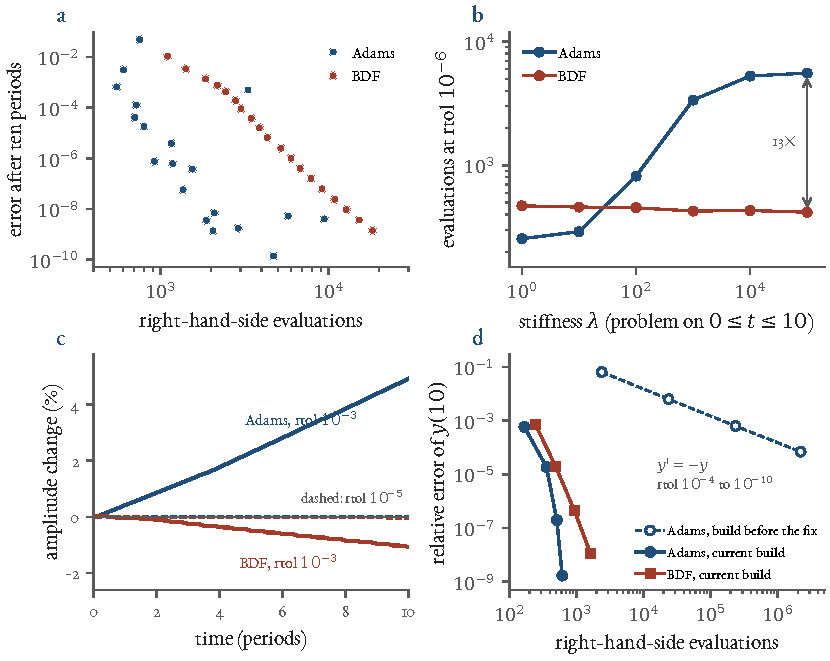
\includegraphics[width=\linewidth]{figures/ch02_workprecision.pdf}
\caption[CVODE on problems with closed-form solutions]{CVODE through the Python module on problems with closed forms; cost is the number of calls of the user's right-hand side, including the finite-difference Jacobian.
(a) Ten periods of $x''=-x$: error against cost, $19$ tolerances each.
(b) Prothero--Robinson problem $y'=-\lambda(y-\cos t)-\sin t$ \cite{ProtheroRobinson1974} on $0\le t\le10$ at $\mathrm{rtol}=10^{-6}$: cost against stiffness $\lambda$.
(c) Amplitude $|(x,v)|$ of the oscillator, exactly $1$, in independent runs to each time: at $\mathrm{rtol}=10^{-3}$ (full lines) and $10^{-5}$ (dashed).
(d) $y'=-y$: the module built on 26 September (before the Adams repair) and the current build.
Script \texttt{figures/ch02\_workprecision.py}; data \texttt{figures/ch02\_numbers.json}, key \texttt{B\_cvode}.}\label{ch02:fig-workprec}
\end{figure}

Panel~(b) is the stiffness test. The Prothero--Robinson problem has the smooth solution $y=\cos t$ for every $\lambda$, and a stiffness that grows with $\lambda$. At $\lambda=1$ Adams is cheaper than BDF ($255$ evaluations against $470$); at $\lambda=10^5$ it is
thirteen times dearer ($5\,565$ against $418$), and BDF's cost has not moved. A fixed-step stability bound would make the Adams cost grow in proportion to $\lambda$; it saturates instead. We did not trace why (a plausible reason is that the order selection falls back
to the A-stable orders 1 and 2, but the Python module does not report the order). What the measurement shows is the textbook division of labour with its cost attached: the non-stiff method is the cheaper one on the non-stiff problem, and an order of
magnitude dearer on the stiff one.

Panel~(c) matters for a Hamiltonian equation like \cref{ch02:eq-pgpe}: the oscillator has a conserved amplitude, as the PGPE has a conserved norm. After ten periods at $\mathrm{rtol}=10^{-3}$ the BDF solution has lost $1.1\,\%$ of its amplitude ($0.043\,\%$ at $10^{-5}$), as a dissipative method does on an oscillation (the stability theory is in
\cite{HairerWanner1996}), and in all $19$ runs of panel~(a) it ended with an amplitude below $1$. Adams errs in either direction depending on the tolerance (negative in $11$ of the $19$ runs); at $\mathrm{rtol}=10^{-3}$ it gained $4.9\,\%$, at $10^{-5}$ $0.004\,\%$. The integrator
has a bias of its own, which competes with the physics being simulated.

Panel~(d) is the defect of the previous section made visible. With the old module the error of Adams on the simplest problem of all, $y'=-y$, falls by a factor $10^{0.5}$ per decade of tolerance while the cost rises by the same
factor, the signature of a first-order method: at $\mathrm{rtol}=10^{-10}$ it needs $2.2\times10^{6}$ evaluations for an error of $6.9\times10^{-5}$, where the current build needs $616$ for $1.7\times10^{-9}$.
Every Adams run made with a build that predates the repair was a run of implicit Euler.

\section{The plane wave: a theorem and three integrators}\label{ch02:planewave}

The known answer is the one proved in \cref{ch02:theorem}. We take a plane wave on a periodic box of side $L=16$, $g=1$, density $1$, wave number $k=2\pi\cdot3/L=1.178$, so that
$\Omega=k^2/2+g=1.694$ (the one-mode form of the theorem is $\dot a=-\ii(k^2/2+g|a|^2)a$ with $|a|=1$), and integrate to $t=10$. The box below shows the call in the Rust engine.

\begin{rustbox}{qf-pgpe against the exact solution}
% CODE snippet2
\begin{lstlisting}[style=py]
import numpy as np, qf_pgpe

N, L, g, m = 32, 16.0, 1.0, 3
engine = qf_pgpe.Pgpe(N, L, g, 0.01)       # grid, box, coupling, time step
x = np.arange(N) * L / N
X, Y = np.meshgrid(x, x, indexing="ij")
k = 2 * np.pi * m / L
psi0 = np.exp(1j * k * X)                  # one mode, density 1
c = engine.run(np.ascontiguousarray(engine.modes(psi0)), 10.0)
omega = 0.5 * k ** 2 + g                   # omega = k^2/2 + g |a0|^2
exact = psi0 * np.exp(-1j * omega * 10.0)
err = np.abs(engine.psi(c) - exact).max()
print(f"plane wave, t = 10: max |psi - exact| = {err:.2e}")
\end{lstlisting}
% OUTPUT snippet2
\begin{lstlisting}[style=plainmono]
plane wave, t = 10: max |psi - exact| = 1.12e-08
\end{lstlisting}
\end{rustbox}

The error is $1.1\times10^{-8}$ at $\Delta t=0.01$. Panel~(a) of \cref{ch02:fig-plane} shows how it arises. For $\Delta t=0.02$, $0.01$, $0.005$ the error at $t=10$ is $1.8\times10^{-7}$, $1.1\times10^{-8}$ and $7.0\times10^{-10}$, in the numpy engine and in the
Rust engine alike (the two final states differ by $4\times10^{-14}$ at most, relative to the amplitude of the occupied mode); the ratios are $15.9$ and $16.0$. The error grows in proportion to $t$ and is a phase error: over the same run the norm of the state, hence the amplitude of the mode, changes by only $7\times10^{-12}$ (relative) at $\Delta t=0.01$; its dependence
on the step is that of a fourth-order scheme. At the programme's registered configuration (known answer K4: $N=64$, $L=32$, $\Delta t=0.005$, $t=10$, acceptance $10^{-9}$) both engines give $7.0\times10^{-10}$, the value of the stored first run. With $g=0$ the error
is $1.1\times10^{-14}$, rounding level.

\begin{figure}[tp]\centering
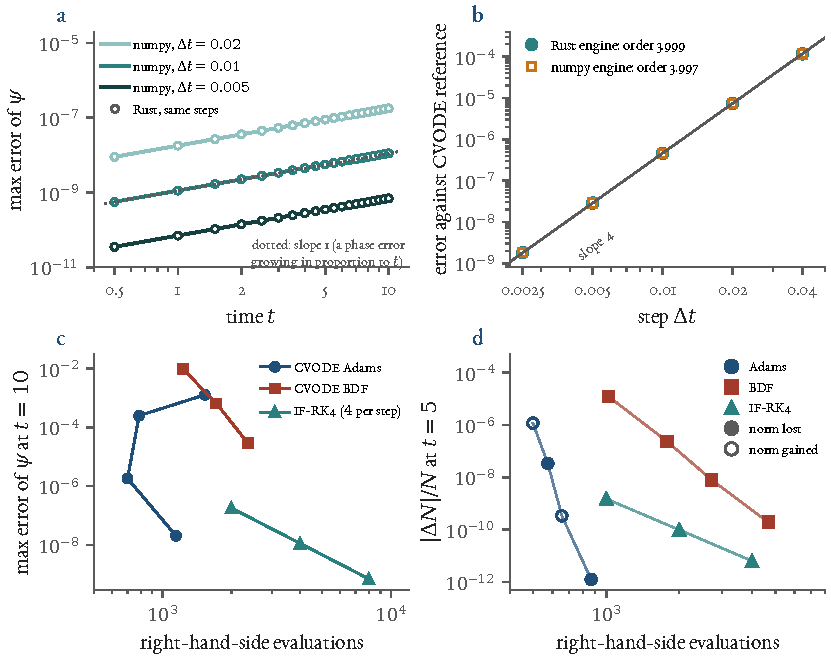
\includegraphics[width=\linewidth]{figures/ch02_planewave.pdf}
\caption[The exact plane wave against three integrators]{The exact plane wave against three integrators. (a) Error of the numpy IF-RK4 engine (lines) and of the Rust engine (circles) against $\psi_0\ee^{-\ii\Omega t}$, $N=32$, three steps; the error grows $\propto t$.
(b) Order of the IF-RK4 step measured against a CVODE (Adams, $\mathrm{rtol}=10^{-12}$) solution of the same right-hand side on a $16\times16$ grid, $t=1$: the registered Rust example (re-run; its output is identical to the stored file)
gives order $3.999$, the same test through the Python module and the numpy engine $3.997$; the errors of the two routes agree to $0.8\,\%$. (c) Cost against accuracy on the $16\times16$ plane wave. (d) Drift of the norm for a state with interacting modes
(a smooth three-mode superposition, $t=5$); filled symbols: norm lost, open: norm gained. Script \texttt{figures/ch02\_planewave.py}; keys \texttt{A\_order}, \texttt{C\_planewave}, \texttt{D\_invariants}.}\label{ch02:fig-plane}
\end{figure}

\paragraph{The order of the scheme, by an independent integrator.} The programme's registered control K2 asks that the energy drift of the scheme fall as $\Delta t^4$. The Rust port tests the order more directly, against a solution of the \emph{same} right-hand side by CVODE,
which shares with the engine nothing but that function. On a $16\times16$ grid ($49$ modes) with a smooth initial state, CVODE (Adams, $\mathrm{rtol}=10^{-12}$, $\mathrm{atol}=10^{-14}$) needs $482$ evaluations in $95$ steps, and the engine's error at $\Delta t=0.04,\dots,0.0025$ falls from $1.2\times10^{-4}$ to $1.8\times10^{-9}$ with successive
ratios $15.99$, $16.00$, $16.00$ and $15.97$ (a fourth-order scheme gives $16$). The fitted order is $3.999$. The reference run needs the Adams repair: with the old path it does not finish.

\paragraph{CVODE on the same wave.} Panel~(c) puts the integrators on one axis, for the $16\times16$ plane wave. CVODE's error is not monotone in its tolerance: Adams with $\mathrm{rtol}=10^{-4}$ spent $1\,530$ evaluations and ended with an error of $1.3\times10^{-3}$, with $10^{-6}$ it spent $788$ and ended with
$2.5\times10^{-4}$, with $10^{-8}$ $701$ and $1.8\times10^{-6}$, with $10^{-10}$ $1\,143$ and $2.0\times10^{-8}$; BDF at $10^{-8}$ spent $2\,364$ for $2.9\times10^{-5}$. At comparable error the engine's scheme needs about three times the
evaluations of CVODE-Adams at its tightest tolerance ($\approx3\,400$ for $2\times10^{-8}$, by interpolation) and, unlike CVODE, its error is monotone in the step. An evaluation of the engine's nonlinear term and one of CVODE's full right-hand side are not the same amount of work, and which integrator is cheaper is not the
point. The point is that all three reproduce the exact solution of the theorem to the precision each promises, which is what ``the program computes the function'' means in this case.

\paragraph{What does not conserve what.} Lean proves that the vector field has zero norm rate. Panel~(d) shows what integrators do with a conserved quantity. On a smooth state with interacting modes (the order-test state, evolved to $t=5$) the relative change of the norm under IF-RK4 at $\Delta t=0.02$, $0.01$, $0.005$ is
$-1.5\times10^{-9}$, $-9.8\times10^{-11}$ and $-6.3\times10^{-12}$: it falls by a factor $15$--$16$ per halving, so it is truncation error, not conservation. For CVODE-Adams at $\mathrm{rtol}=10^{-4}$ to $10^{-10}$ it is $+1.2\times10^{-6}$, $-3.4\times10^{-8}$,
$+3.3\times10^{-10}$ and $-1.2\times10^{-12}$, of either sign. For BDF it is $-1.2\times10^{-5}$, $-2.3\times10^{-7}$, $-7.9\times10^{-9}$ and $-1.9\times10^{-10}$, always a loss. No integrator conserves the norm; each
loses or gains it at a rate set by its own tolerance. The theorem is about the equation, and is true; the invariant is conserved by the program to a stated precision and no further.

\section{Where a theorem and a program part: aliasing}\label{ch02:alias}

The engine does not evaluate $N_k$ of \cref{ch02:eq-modes}. It evaluates $P[\,\mathrm{FFT}(|\psi|^2\psi)\,]$ on an $N\times N$ grid: transform to the grid, cube pointwise, transform back, keep the modes inside the projector. On the grid a
wave vector is a class modulo $N$, so a triple with $k_1-k_2+k_3=k+Nm$ for an integer vector $m\ne0$ is added to the same output mode as the triples with $m=0$. The engine's cubic term is a sum over all triples whose sum is congruent to $k$; the
Lean $N_k$ is a sum over the triples whose sum \emph{is} $k$. They are the same function exactly when no triple wraps.

The box below is the check: a literal transcription of the Lean definition for $G=\mathbb Z^2$, no wrap-around, and a comparison with the numpy engine's cubic term, rescaled to the units of the Lean statement ($a=c/N^2$ for the unnormalized FFT
convention of the engine). The transcription was written for this chapter and is not checked by Lean; its consistency is tested below.

\begin{rustbox}{The Lean definition of the cubic term, transcribed, against the engine}
% CODE lean_nl
\begin{lstlisting}[style=py]
def lean_nl(Lam, A):
    """Literal transcription of QuantumFluids.GPGalerkin.nl on Z^2:
         nl psi k = sum over k1, k2, k3 in Lam with k1 + k3 = k + k2 of
                    psi k1 * conj(psi k2) * psi k3        (no wrap-around)
       Lam: (m, 2) integer array of modes, A: (m,) amplitudes psi.
       Returns (table, B) with table[kx + B, ky + B] = nl psi (kx, ky)."""
    m = len(Lam)
    B = 3 * int(np.abs(Lam).max()) + 1               # sums reach 3 R
    size = 2 * B + 1
    re = np.zeros(size * size)
    im = np.zeros(size * size)
    for i in range(m):                               # k1 = Lam[i]
        k = Lam[i] - Lam[:, None, :] + Lam[None, :, :]       # k1 - k2 + k3
        idx = ((k[..., 0] + B) * size + (k[..., 1] + B)).ravel()
        v = (A[i] * np.conj(A)[:, None] * A[None, :]).ravel()
        re += np.bincount(idx, weights=v.real, minlength=size * size)
        im += np.bincount(idx, weights=v.imag, minlength=size * size)
    return (re + 1j * im).reshape(size, size), B
\end{lstlisting}
and, in the driver, the engine's term in the same units:
% CODE engine_vs_lean
\begin{lstlisting}[style=py]
a = np.zeros((N, N), dtype=complex)
a[s.P] = A                  # psi_k, the units of the Lean statement
c = a * N ** 2              # the engine's unnormalized FFT amplitudes
# the engine's cubic term, in the units of nl:
nl_eng = s.nonlin(c) / (-1j * g * N ** 2)
\end{lstlisting}
% OUTPUT snippet3
\begin{lstlisting}[style=plainmono]
cutoff 0.500  modes 197  max|engine-nl|/max|nl| = 7.85e-16  differing: 0
cutoff 0.500  modes 197  max|engine-nl|/max|nl| = 1.15e-03  differing: 4
cutoff 0.667  modes 357  max|engine-nl|/max|nl| = 1.53e-01  differing: 348
\end{lstlisting}
The three lines are the cases of \cref{ch02:fig-bridge,ch02:fig-rates}: $N=32$, $L=16$, a random complex state on the retained modes (seed fixed); the first with the four extreme modes empty, the second with all modes filled, the third at the larger cutoff.
Function \texttt{lean\_nl} and driver \texttt{bridge\_case} of \texttt{figures/ch02\_compute.py}, run by \texttt{figures/ch02\_snippets.py}.
\end{rustbox}

With the cutoff at one half of the largest wave number, the engine's cubic term equals the Lean definition to $7.9\times10^{-16}$, rounding, on a state whose four extreme modes are empty. With those modes filled, four modes of the $197$ differ, by
$1.1\times10^{-3}$ at most (relative to the largest value of $N_k$). At two thirds, $348$ of $357$ modes differ, by up to $15\,\%$ of the largest value. The geometry of \cref{ch02:fig-bridge}(a,b) explains all three. A triple reaches $|k_1-k_2+k_3|\le3R$ if the retained modes lie in a disc of radius $R$
(in index units); the periodic images of that reach-disc, displaced by $N$ along the axes, intrude into the retained disc when $3R+R>N$. So the engine's function equals $N_k$ for \emph{every} state when $4R<N$, that is, $k_{\rm cut}<k_{\max}/2$. At $4R=N$, which is the engine's
default cutoff, the discs touch at four points: the four modes $\pm(N/4,0)$, $\pm(0,N/4)$, each fed by a single wrapped triple, for the mode $(-N/4,0)$ the triple $k_1=k_3=-k_2=(N/4,0)$, as the data show. For a quadratic nonlinearity the reach is $2R$, the condition is $3R\le N$, and
one recovers the two-thirds rule \cite{Orszag1971}; for the cubic term of the PGPE that rule is wrong, as the programme found.

\begin{figure}[tp]\centering
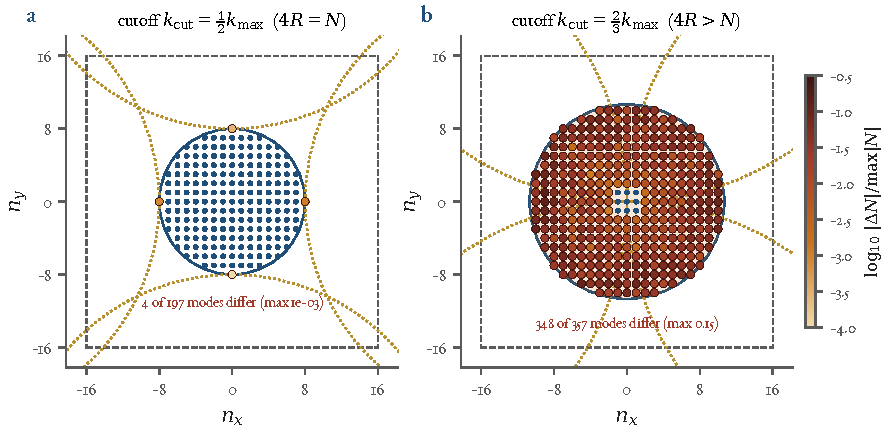
\includegraphics[width=\linewidth]{figures/ch02_bridge.pdf}
\caption[The same equation in the two languages]{The same equation in the two languages: where the engine's cubic term and the literal Lean definition coincide. Retained modes in the index plane ($N=32$), coloured by the difference between the two on a random state with all modes filled; blue: equal to rounding.
Dashed square: the Nyquist box; dotted arcs: the periodic images of the disc of radius $3R$ reached by the triple sums; orange shading: the modes the images cover. The cutoffs are $\frac12k_{\max}$ (a) and $\frac23k_{\max}$ (b).
Script \texttt{figures/ch02\_bridge.py}; key \texttt{E\_bridge}.}\label{ch02:fig-bridge}
\end{figure}



Panel~(a) of \cref{ch02:fig-rates} puts the theorems against the engine. For the literal definition both rates vanish to rounding (below $10^{-17}$ relative to the sum of the moduli of the terms) in all three cases, as \Lthm{GPGalerkin}{mass_rate_zero} and \lean{momentum\_rate\_zero} say they must.
That the transcription is the Lean object is tested by the identity of \Lthm{GPGalerkin}{pairing_eq_sum}, which the transcription satisfies: $Q=1.403114631989707$ against $\sum_q|A_q|^2=1.4031146319897068$, with imaginary part $2.8\times10^{-17}$.
For the engine, the mass rate is zero to rounding even where triples wrap: by Parseval on the grid
\[
\sum_k\overline{a_k}\,P\bigl[\mathrm{FFT}(|\psi|^2\psi)\bigr]_k=\sum_x|\psi(x)|^4 ,
\]
a real number, wrapped or not (an argument, not a Lean theorem). The momentum rate is not zero: $1.6\times10^{-17}$ with the extreme modes empty, $2.3\times10^{-5}$ with them filled, $4.1\times10^{-3}$ at the larger cutoff.
The theorem and the program agree exactly where the theorem's hypothesis holds, and part company where it does not: there the grid is $\mathbb Z_N^2$, and \lean{no\_momentum\_on\_torus} says that no additive momentum exists on it.

\begin{figure}[tp]\centering
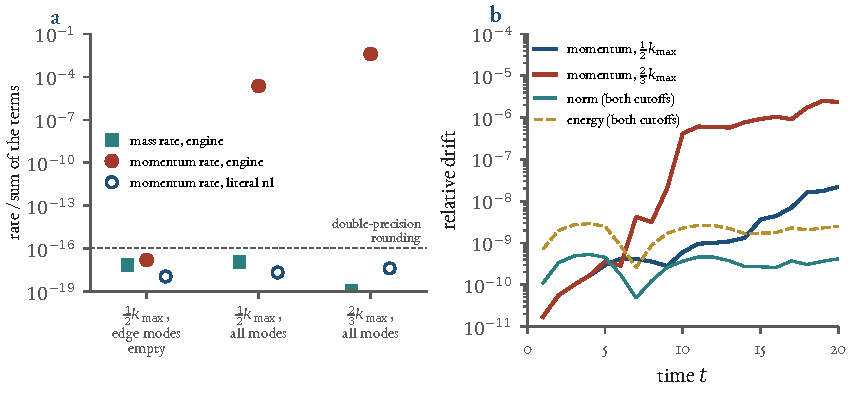
\includegraphics[width=\linewidth]{figures/ch02_rates.pdf}
\caption[Theorems and engine, in rates and in time]{Theorems and engine, in rates and in time. (a) Instantaneous rates for the engine and for the literal definition, in the three cases of the text: of the mass, $|\sum_k\mathrm{Im}(\overline{\psi_k}G_k)|\big/\sum_k|\overline{\psi_k}G_k|$, and of the momentum, the same with the weight $p(k)=k_x$ in numerator and
denominator; the Lean theorems say that the literal definition gives zero. The point on the lower edge is exactly $0$. (b) Drift of the invariants along an IF-RK4 run ($\Delta t=0.01$) from one smooth random state at $N=32$, for the two cutoffs; norm and energy are the same for both.
Script \texttt{figures/ch02\_bridge.py}; key \texttt{E\_bridge}.}\label{ch02:fig-rates}
\end{figure}

Integrated in time (panel~(b) of \cref{ch02:fig-rates}), one smooth random state ($N=32$, $L=16$, energy $0.6$ per particle, seed $3$) evolved by IF-RK4 at $\Delta t=0.01$ with the two cutoffs has at $t=10$ a relative norm drift of $3.7\times10^{-10}$ and an energy drift of $2.3\times10^{-9}$, the same at both cutoffs,
and a momentum drift (relative to $\sum_k|k||c_k|^2$) of $6.0\times10^{-10}$ at $\frac12k_{\max}$ and $4.2\times10^{-7}$ at $\frac23k_{\max}$; at $t=20$ the momentum drifts are $2.2\times10^{-8}$ and $2.4\times10^{-6}$, norm and energy $4.2\times10^{-10}$ and $2.5\times10^{-9}$ for both. Norm and energy do not see the aliasing;
momentum does, separating the two cutoffs by two to three orders of magnitude. This is a modest reproduction of the programme's control, on a smooth state and a $32^2$ grid where the recorded failure ($8.5$, one per cent) was a random high-energy state on $64^2$. The drift at the one-half cutoff is not zero either; we did not separate the
truncation error of the scheme from the effect of the four edge modes, which the evolving state may populate.

\section{What each instrument can see}\label{ch02:see}

\Cref{ch02:tab-see} sorts the statements of this chapter by the instrument that can establish them. The rows for the norm and the plane wave are the reason the programme runs controls of several kinds: a proof of the right theorem cannot detect that the program evaluates another function, and the control that
can, the momentum, is one that the norm and the plane wave are blind to.

\begin{table}[t]\centering\footnotesize
\begin{tabular}{p{0.14\linewidth}p{0.24\linewidth}p{0.30\linewidth}p{0.19\linewidth}}\toprule
property & Lean (a statement for every $\Lambda$ and state) & registered control and independent integrators & what it caught here\\\midrule
norm rate $=0$ & \lean{mass\_rate\_\allowbreak zero} (library), any $\Lambda$ & K1: drift $4.2\times10^{-10}$; engine rate at most $1.1\times10^{-17}$ in all cases & nothing: blind to aliasing\\
exact plane wave & \lean{planeState\_\allowbreak solves\_\allowbreak galerkin} (new) & K4: $7.0\times10^{-10}$; numpy, Rust and CVODE agree & nothing: blind to aliasing\\
momentum rate $=0$ & \lean{momentum\_\allowbreak rate\_\allowbreak zero} (new), needs an additive $p$ & K3: drift $8.5$ in the first run; rate $4.1\times10^{-3}$ at $\frac23k_{\max}$ & the wrong cutoff rule\\
order of IF-RK4 & none in the library & K2 (energy drift $\propto\Delta t^4$); error against CVODE: order $3.999$ & the Adams defect: the reference run cannot finish without the repair\\
the program computes the function & none: a statement about a program & transcription of \lean{nl} against the engine & $4$ modes differ at $\frac12k_{\max}$, $348$ at $\frac23k_{\max}$\\\bottomrule
\end{tabular}
\caption{Which instrument can establish what. The first two controls pass with or without aliasing; the third separates the cutoffs.}\label{ch02:tab-see}
\end{table}

\begin{honestbox}
\begin{itemize}
\item \textbf{Proved} (Lean, kernel-checked, standard axioms only). For every finite mode set in every additive group: the mass-rate identity and the non-negativity of the quartic interaction (library, \lean{GPGalerkin}); the exact plane wave solves the
Galerkin system; the momentum-rate identity for every additive weight; no non-zero additive map exists on $\mathbb Z_N\times\mathbb Z_N$ (new, \texttt{book/lean/Ch02\_Galerkin.lean}). These are statements about the mathematical function $N_k$ and about rates at an instant: not about existence of solutions,
not about conservation along a solution, not about any program.
\item \textbf{Measured or simulated.} The engine's cubic term equals a transcription of $N_k$ to $8\times10^{-16}$ when no triple wraps (one random state per case, $N=32$); three integrators reproduce the exact plane wave to the precisions stated; the order of the IF-RK4 step is $4.00$ (fitted $3.999$ and $3.997$);
CVODE's costs and errors on the stated problems, with the build described above.
\item \textbf{Not established.} That the transcription equals the Lean object is a correspondence made by hand and tested by one identity, not proved; nothing proves the Rust code; agreement of rusty-SUNDIALS with the C library is not claimed; the stability regions are fixed-step guides; the Adams cost on the stiff problem is
measured but its cause is not traced; the momentum drift at the one-half cutoff mixes truncation error and edge-mode aliasing, which we did not separate.
\item \textbf{An analogy, not a result.} The division into ``Lean sees'' and ``the solver sees'' is a classification of this chapter's cases, not a theorem about methods.
\item \textbf{What failed.} The pre-registered rule $k_{\rm cut}=\frac23k_{\max}$ was wrong for a cubic term, and the momentum control caught it. The pre-registration's sentence that the three conservation laws were library theorems was wrong for one of them and incomplete for the other two.
The Adams path of rusty-SUNDIALS was implicit Euler until it was repaired, and the module in the programme's virtual environment still is. The first draft of this chapter's Lean file contained a proof that did not compile, and its audit line carried \lean{sorryAx}.
\end{itemize}
\end{honestbox}

\paragraph{Exercise 1.} In a commutative ring with $e^3=0$ show that $(1+e)(1-e+e^2)=1$ by \lean{linear\_combination}, then change the sign of the $e^2$ term and read the reply. \emph{Hint.} The goal minus the coefficient times the hypothesis must be an identity of rings: $(1+e)(1-e+e^2)-1=e^3$, so the coefficient is $1$.

\paragraph{Exercise 2.} In the first box of \cref{ch02:solver} replace the oscillator by the Prothero--Robinson problem with $\lambda=10^4$: right-hand side \lean{[-lam * (y[0] - math.cos(t)) - math.sin(t)]}, initial value \lean{[1.0]}, end time $10$, tolerances \lean{1e-6} and \lean{1e-8}.
Count the calls for both methods and compare with \cref{ch02:fig-workprec}(b); then set \lean{max\_steps} to $300$ and read the reply. \emph{Hint.} With the build used here the counts are $5\,270$ (Adams) and $431$ (BDF). With \lean{max\_steps = 300} BDF still finishes, and Adams stops with
\lean{maximum steps exceeded (300) at t=1.77}: \lean{max\_steps} counts internal steps, and Adams needs more than $300$ of them for the first $1.8$ time units.

\paragraph{Exercise 3.} (a) On a grid with $N=16$ the retained set at $k_{\rm cut}=\frac12k_{\max}$ contains $(\pm4,0)$ and $(0,\pm4)$. Find the single wrapped triple that feeds the mode $(-4,0)$, and use the geometry of \cref{ch02:fig-bridge} to say for which cutoffs the cubic term of the engine equals $N_k$ for \emph{every} state
when $N=16$ (answer in index units). (b) Show that the engine's mass rate $\sum_k\mathrm{Im}(\overline{a_k}G_k)$ vanishes for every state, wrapped or not, and explain why the same argument cannot give momentum.
\emph{Hint.} (a) Look for $k_1+k_3-k_2=(-4,0)+(16,0)$ with all three modes of norm $4$; the condition is $4R<N$. (b) Parseval on the grid turns $\sum_k\overline{a_k}P[\mathrm{FFT}(|\psi|^2\psi)]_k$ into $\sum_x|\psi(x)|^4$; for momentum you need a function of $k$ that is additive modulo $N$, and \lean{no\_momentum\_on\_torus} says there is none.

\section{Notes and further reading}\label{ch02:notes}

For Lean, \emph{Theorem Proving in Lean~4} \cite{TPIL4} introduces the language and \emph{Mathematics in Lean} \cite{MIL} the use of Mathlib; the kernel and the elaborator are described in \cite{deMoura2021}. For the numerics, Hairer, N{\o}rsett and Wanner \cite{HairerNorsettWanner1993} treat Adams methods and
Hairer and Wanner \cite{HairerWanner1996} stiffness, BDF and absolute stability, with Dahlquist's paper on A-stability \cite{Dahlquist1963} as the source of the notion; Prothero and Robinson \cite{ProtheroRobinson1974} define the stiff test problem used here; the SUNDIALS suite is described in \cite{Hindmarsh2005}. The
pseudo-spectral treatment of the projected equation and the aliasing rules are in \cite{Blakie2008} and \cite{Orszag1971}. The solver is described, with its cross-checks and its performance, in the software paper \cite{Callens2026sw}, the Lean library in \cite{Callens2026lib}. Everything in this chapter can be regenerated: the numbers by
\texttt{figures/ch02\_compute.py} (parts A to E, into \texttt{figures/ch02\_numbers.json}), the code boxes by \texttt{figures/ch02\_snippets.py}, the figures by the four \texttt{figures/ch02\_*.py} scripts, the Lean files with
\texttt{lake env lean} on the three files \texttt{book/lean/Ch02\_*.lean}; the Python module of the current build is made by \texttt{book/rust/ch02\_build\_py.sh} (the copy used here, with its checksum, is in \texttt{/mnt/data/xdev-cache/rs\_py\_5db8041}). The next chapters use the two languages without
re-introducing them; \cref{ch10} returns to the question of how far each instrument can be trusted.
